\documentclass[11pt, a4paper]{article}
\sloppy %prevents text from going over the right margin
% \usepackage[T1]{fontenc}
\usepackage[utf8]{inputenc}
\usepackage{listings}
\usepackage[margin=1.0in]{geometry}
\usepackage{color}
\usepackage{graphicx}
\usepackage{tabularx}
\usepackage{url}
\usepackage[normalem]{ulem} 
\usepackage{enumitem}
\usepackage{hyperref}
\usepackage{fancyhdr} %Package to configure headings and footer
\usepackage{lastpage}
\usepackage{gensymb}
\usepackage[version=3]{mhchem}
\usepackage[ngerman]{babel}
\setlength\parindent{0pt}

\newcommand{\VARtitle}{NW2}
\newcommand{\VARauthor}{Janeczek}

\title{Ozon \\ \VARtitle}
\author{\VARauthor}
\date{\today{}, Vienna}

% header
\pagestyle{fancy}
\fancyhead[L]{\today}
\fancyhead[R]{\VARtitle}

%footer
\fancyfoot[L]{\VARauthor}
\fancyfoot[C]{5AHITT}
\fancyfoot[R]{Page \thepage/\pageref{LastPage}}


\begin{document}

\lstset{ %
  backgroundcolor=\color{white},   % choose the background color; you must add \usepackage{color} or \usepackage{xcolor}
  basicstyle=\footnotesize,        % the size of the fonts that are used for the code
  breakatwhitespace=false,         % sets if automatic breaks should only happen at whitespace
  breaklines=true,                 % sets automatic line breaking
  captionpos=b,                    % sets the caption-position to bottom
% commentstyle=\color{mygreen},    % comment style
  deletekeywords={...},            % if you want to delete keywords from the given language
  escapeinside={\%*}{*)},          % if you want to add LaTeX within your code
  extendedchars=false,              % lets you use non-ASCII characters; for 8-bits encodings only, does not work with UTF-8
% frame=single,                    % adds a frame around the code
  keepspaces=true,                 % keeps spaces in text, useful for keeping indentation of code (possibly needs columns=flexible)
% keywordstyle=\color{blue},       % keyword style
% language=bash,                   % the language of the code
  morekeywords={*,...},            % if you want to add more keywords to the set
  numbers=left,                    % where to put the line-numbers; possible values are (none, left, right)
  numbersep=5pt,                   % how far the line-numbers are from the code
  rulecolor=\color{black},         % if not set, the frame-color may be changed on line-breaks within not-black text (e.g. comments (green here))
  showspaces=false,                % show spaces everywhere adding particular underscores; it overrides 'showstringspaces'
  showstringspaces=false,          % underline spaces within strings only
  showtabs=false,                  % show tabs within strings adding particular underscores
  stepnumber=1,                    % the step between two line-numbers. If it's 1, each line will be numbered
  tabsize=2,                       % sets default tabsize to 2 spaces
  title=\lstname                   % show the filename of files included with \lstinputlisting; also try caption instead of title
}


\maketitle
\newpage
\tableofcontents
\newpage


\section{Vorwort}

In diesem Dokument wird eine meiner naturwissenschaftlichen Thematiken ausgearbeitet. Es handelt sich um den Fachbereich der Meteorologie. Ich werde euch einen wesentlichen Überblick bezüglich des Moleküls Ozon, dem Ozonloch und dessen Entstehung liefern.

\section{Ozon}

\subsection{Begriffserklärung}
\textbf{Was versteht man unter Ozon?}\\
Ozon ist ein gasförmiges Molekül, das in kleinsten Mengen in unserer Atemluft vorkommt. Es handelt sich um ein starkes Oxidationsmittel, jedoch führt es bei Menschen und Tieren zu Reizungen der Atemwege. \\

\begin{figure}[h!]
	\centering
	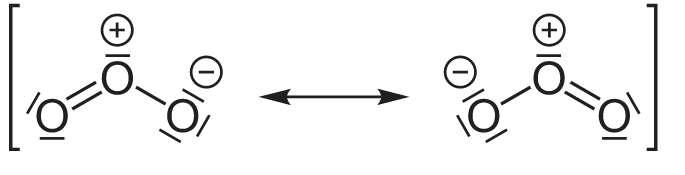
\includegraphics[width=0.8\textwidth]{images/ozon}
	\caption{Mesomere Grenzstrukturen des Ozonmoleküls}
\end{figure}

\subsection{Entstehung}
\textbf{Wie bildet sich Ozon?}\\
Prinzipiell sind uns drei Arten der Entstehung von Ozon bekannt:
\subsubsection{Entstehung durch Sauerstoff}
Ozon entsteht an sich aus gewöhnlichem Sauerstoff und einiger Vorläufersubstanzen (Kohlenwasserstoffe VOC und Stickstoffdioxid NO2). Je mehr VOC und NO2 in der Luft vorkommen und je stärker die Sonne scheint, umso mehr Ozon wird gebildet. Im Wesentlichen ist der Straßenverkehr für die Bildung von Ozon verantwortlich (NO2 kommt weitgehend aus dem motorisiertem Verkehr, VOC aus dem motorisierten Verkehr, Industrie, Gewerbe, Haushalte). 
\subsubsection{Enstehung durch energiereiche Sonnenstrahlung}
Die in der Stratosphäre (~50km) befindlichen Sauerstoff-Moleküle werden in zwei einzelne Sauerstoff-Partikel gespalten. Diese vereinigen sich mit anderen Sauerstoff-Molekülen wieder zu Ozon.
\subsubsection{Entstehung durch Gewitter}
Durch den eelektrischen Stromfluss zwischen Wolke und Erdboden entsteht bei der Blitzentladung Ozon sowie andere Schadstoffe (z.B. Salpetersäure).

\newpage
\subsection{Auswirkungen}
\textbf{Welche Auswirkungen hat Ozon?}\\
In hohen Konzentrationen gefährdet Ozon die Gesundheit von Menschen, Tieren und Pflanzen. Ozon an sich ist schlecht wasserlöslich, dringt tief in die Lungen ein und kann dort Zellreizungen hervorrufen. Das Element greift aufgrund seiner stark oxidierenden, aggressiven Eigenschaften auch Sachgüter an. Nach Kohlendioxid und Methan trägt Ozon als drittwichtigstes anthrophogene (=von Menschen verursacht, entstanden, ...) Gas zur Klimaerwärmung bei. \\

Eintreffende Ultraviolettstrahlung/UV-Photonen schädigen außerdem die DNA und beschädigte Hautzellen sind Krebszellen.

\begin{figure}[h!]
	\centering
	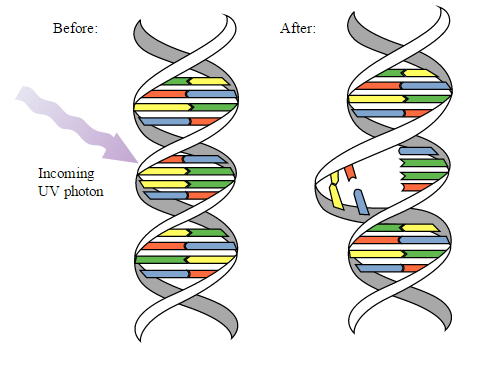
\includegraphics[width=0.8\textwidth]{images/dna}
	\caption{UV-Photonen schädigen die DNA}
\end{figure}

\textbf{Wie profitieren wir von Ozon?}\\
Bisher wurden nur Nachteile des aggressiven Gases genannt. Die Sache ist nämlich, dass wir ohne Ozon nicht leben könnten.\\ \\ Hierfür ist die sogenannte Ozonschicht, die sich in der Stratosphäre befindet und sich über 20km Dicke erfreut, verantwortlich. Dieses von unserem Planeten entfernte Ozon umhüllt die Erde wie ein gigantischer Schutzschild und schirmt unseren Planeten vor dem gefährlichen Ultraviolettstrahlen der Sonne ab. Ohne der Ozonschicht wären wir also neben Sonnendbränden auch von Hautkrebs und Schädigungen der Augen gefährdet. \\ \\
Ozon ist lichtempfindlicher als das uns bekannte Sauerstoff-Molekül O2. Es absorbiert UV-C und UV-B und schützt damit jegliche Lebensform vor Strahlungsschäden. \\ \\
Wenn ein Ozon Molekül ein UV-Photon absorbiert, wird es gespalten, aber in den allermeisten Fällen bildet das freigesetzte O-Partikel sofort wieder Ozon. \\

\newpage
\begin{center}
Das Sauerstoff-Molekül wird durch Sonnenstrahlen gespalten. \\
\ce{O2 ->C[hv] O + O} \\
Die dadurch entstandenen Sauerstoff-Partikel bilden mit Sauerstoff-Molekülen wieder Ozon. \\
\ce{O + O2 -> O3} \\
Aufspaltung des Ozons + Rückbildung \\
\ce{O3 ->C[hv] O2 + O} \\
\end{center}

\section{Ozonloch}
\subsection{Begriffserklärung}
Über der Antarktis (und neuerdings über der Arktis) stellt sich seit 15 Jahren zu bestimmten Zeit des Jahres ein Verlust an straospährischem Ozon ein. Der Grund dafür sind menschengemacht Chemikalien, welche Chlor enthalten, insbesondere FCKWs (Fluor-Chlor-Kohlenwasserstoffe) aber auch Stickoxide(NOx). FCKWs sind ein weit verbreitetes Erzeugnis, welches in Kühlsystemen, Klimaanlagen, als Treibgas und Lösungsmittel Verwendung findet.

\begin{figure}[h!]
	\centering
	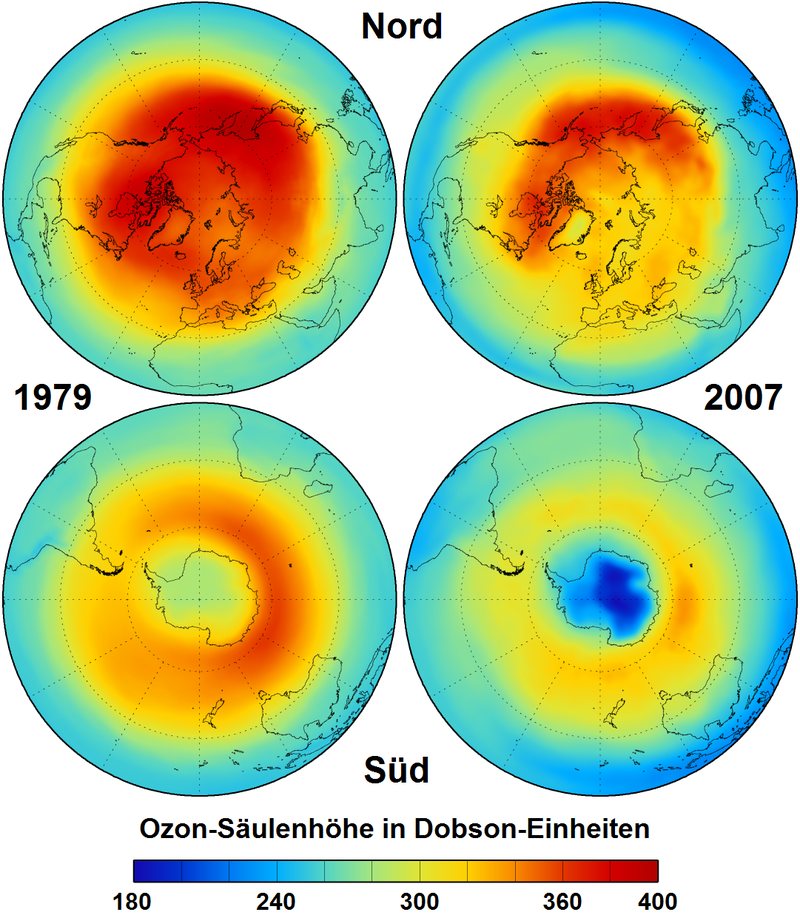
\includegraphics[width=0.65\textwidth]{images/ozondichte}
	\caption{Ozonschichtdicke 1979 und 2007}
\end{figure}

\newpage
\subsection{Vorgehensweise gegen das Ozonloch}
Das Protokoll von Montreal, welches im Jahr 1987 unterzeichnet wurde, zielt auf die Begrenzung der FCKWs ab und will diese bis zum Jahre 2000 halbieren. Die industrielle Produktion vieler Hologen-Kohlenstoffe soll bis 2030 kontrolliert werden. Die wichtigsten FCKWs sollen ab Anfang 1995 nicht mehr produziert werden. \\
Das wesentliche Problem ist, dass die Erholung des in der Stratosphäre befindlichen Ozons sehr viel Zeit in Anspruch nimmt (~30 bis 50 Jahre).
\subsection{Ozonloch an den Polen}
\textbf{Wieso ist das Ozonloch an den Poln am dünnsten?}\\
Wiee bereits erläutert, gibt es Radikale, die deen Zerfall von Ozon beschleunigen. \\Einige davon sind natürlicher Herkunft, andere werden von uns Menschen in die Atmosphäre geblasen (z.B. Chlor). Ein Radkial zerstört mehrere Ozonmoleküle (im Bereich von 1:1000). \\Der Zyklus kann nur unterbrochen werden, wenn die Radikale eine feste Bindung eingehen, indem sie mit anderen Stoffen, wie zum Beispiel Stickstoffdioxid reagieren.

\begin{figure}[h!]
	\centering
	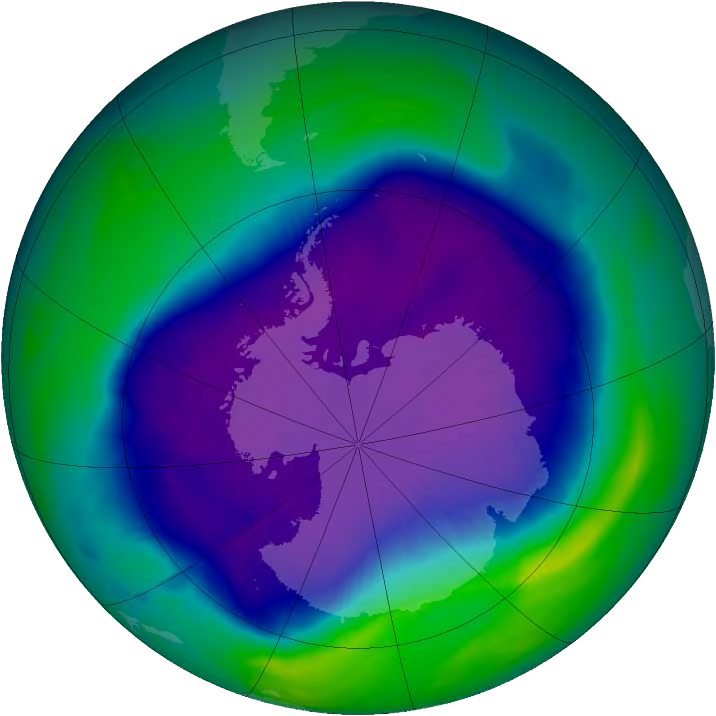
\includegraphics[width=0.5\textwidth]{images/ozonloch}
	\caption{Bisher größte Ausdehnung des antarktischen Ozonlochs am 24. September 2006}
\end{figure}

Der Grund warum bei der Antarktis ein erhöhter Ozonabbau stattfindet, ist die enorme, die während der Polarnacht auftritt. \\ \\Aufgrund dieser Kälte werden einige Radikalverbindungen wieder getrennt, das bedeutet es sind mehr Radikale für die Zerstörung des Ozons übrig. Erst wenn diese 'Wolken', die wegen der Kälte entstanden sind, wieder verdampfen kann der Ozonabbau gedämpft werden. 
\newpage
\nocite{*}
\bibliographystyle{plain}
\bibliography{bibliography}{}

\end{document}